\section{Overlapping Periods}

In addition to the areas of coexistence of cycles of the same period, discussed above, there are also areas of coexistence, where cycles of different periods coexist.
\Cref{fig:yunus.period.regions} shows the edges of regions of the same period when scanned from different directions.
The scan from left to right is colored in yellow, and from right to left in purple.
At most points, they agree with the corresponding scans from top to bottom in red and from bottom to top in blue, respectively.
When starting in an area of coexistence, blue, purple, yellow, and red show some disagreements.
This is apparent in the zoomed-in \Cref{fig:yunus.period.regions.zoomed}.
This is because the cycles sometimes start on one period and sometimes on another.
When the scans start in an area, where just one period exists, they agree for the most part.
There is another exception, that is the scans from top to bottom in red and from bottom to top in blue can't detect the ``teeth'' because they lose the cycles at an earlier edge.

\begin{figure}
    \centering
    \begin{subfigure}{0.4\textwidth}
        \includegraphics[width=\textwidth]{99_Yunus/2D_Regions_Zoomed/result.png}
        \caption{Overview}
        \label{fig:yunus.period.regions}
    \end{subfigure}
    \begin{subfigure}{0.4\textwidth}
        \includegraphics[width=\textwidth]{99_Yunus/2D_Regions_Zoomed2/result.png}
        \caption{Zoomed In}
        \label{fig:yunus.period.regions.zoomed}
    \end{subfigure}
    \caption{Overlapping Areas of Different Periods}
\end{figure}

We can use the same procedure on the same model $\mod \pi$ as we did before, to visualize the edges of ``type A'' and ``type B'' parameter regions.
\Cref{fig:yunus.halved.period.regions.zoomed} shows this for the zoomed-in scan from above.
You can see there that the ``type A'' and ``type B'' parameter regions overlap.
This means that there are parameter regions where there are 3 coexisting stable cycles.

\begin{figure}
    \centering
    \includegraphics[width=0.6\textwidth]{98_Yunus_modpi/2D_Regions_Zoomed2/result.png}
    \caption{Overlapping Areas of Different Periods in Halved Original Model}
    \label{fig:yunus.halved.period.regions.zoomed}
\end{figure}
